\documentclass[11pt,a4paper,oneside]{report}


% Make bibliography appear in table of contents
\usepackage[nottoc,numbib]{tocbibind}

\usepackage{amsmath,amssymb,calc,ifthen,capt-of}

\usepackage{float}

\usepackage[ampersand]{easylist}

\usepackage[table,usenames,dvipsnames]{xcolor} % for coloured cells in tables

\usepackage{tikz}

% Allows us to click on links and references!

\usepackage{hyperref}
\hypersetup{
    colorlinks,
    citecolor=black,
    filecolor=black,
    linkcolor=black,
    urlcolor=black
}

% Nice package for plotting graphs
% See excellent guide:
% http://www.tug.org/TUGboat/tb31-1/tb97wright-pgfplots.pdf
\usepackage{pgfplots}
\usetikzlibrary{plotmarks}
\usepackage{amsmath,graphicx}
\usepackage{epstopdf}
\usepackage{caption}
\usepackage{subcaption}

\pgfplotsset{compat = newest}

% highlight - useful for TODOs and similar
\usepackage{color}
\newcommand{\hilight}[1]{}%\colorbox{yellow}{#1}}


% margin size
\usepackage[margin=1in]{geometry}

\tikzstyle{state}=[circle,thick,draw=black, align=center, minimum size=2.1cm,
inner sep=0]
\tikzstyle{vertex}=[circle,thick,draw=black]
\tikzstyle{terminal}=[rectangle,thick,draw=black]
\tikzstyle{edge} = [draw,thick]
\tikzstyle{lo} = [edge,dotted]
\tikzstyle{hi} = [edge]
\tikzstyle{trans} = [edge,->]

\begin{document}
\belowdisplayskip=12pt plus 3pt minus 9pt
\belowdisplayshortskip=7pt plus 3pt minus 4pt


\Large{\textbf{Coursework Two Results by Razvan Valentin Marinescu}}


\section*{Problem 1}

\begin{table}[H]
  \centering
  The dependency Matrix for the HepatitisC data set:\\
   \ \\
  \begin{tabular}{ c | c | c | c | c | c | c | c | c | c | }
    Variable & 0 & 1 & 2 & 3 & 4 & 5 & 6 & 7 & 8\\
    \hline
    0 & 1.530 & 0.045 & 0.026 & 0.048 & 0.034 & 0.024 & 0.039 & 0.086 & 0.016\\
    \hline
    1 & 0.045 & 2.372 & 0.009 & 0.060 & 0.069 & 0.030 & 0.071 & 0.083 & 0.003\\
    \hline
    2 & 0.026 & 0.009 & 0.992 & 0.012 & 0.007 & 0.002 & 0.007 & 0.005 & 0.001\\
    \hline
    3 & 0.048 & 0.060 & 0.012 & 1.697 & 0.539 & 0.275 & 0.032 & 0.032 & 0.006\\
    \hline
    4 & 0.034 & 0.069 & 0.007 & 0.539 & 2.411 & 0.606 & 0.041 & 0.051 & 0.008\\
    \hline
    5 & 0.024 & 0.030 & 0.002 & 0.275 & 0.606 & 1.832 & 0.025 & 0.041 & 0.016\\
    \hline
    6 & 0.039 & 0.071 & 0.007 & 0.032 & 0.041 & 0.025 & 2.629 & 0.063 & 0.004\\
    \hline
    7 & 0.086 & 0.083 & 0.005 & 0.032 & 0.051 & 0.041 & 0.063 & 1.489 & 0.032\\
    \hline
    8 & 0.016 & 0.003 & 0.001 & 0.006 & 0.008 & 0.016 & 0.004 & 0.032 & 0.754\\
    \hline
  \end{tabular}
%  \caption{}
%  \label{tab:ranks_table}
\end{table}


\section*{Problem 2}


\begin{table}[H]
  \centering
  Dependency List for the HepatitisC data set (descending order):\\
  \ \\
  \begin{tabular}{| c | c | c |}
    \hline
    Dependency & Node \#1 & Node \#2\\
    \hline
    0.60581 & 5 & 4 \\
    \hline
    0.53890 & 4 & 3 \\
    \hline
    0.27452 & 5 & 3 \\
    \hline
    0.08611 & 7 & 0 \\
    \hline
    0.08255 & 7 & 1 \\
    \hline
    0.07137 & 6 & 1 \\
    \hline
    0.06883 & 4 & 1 \\
    \hline
    0.06294 & 7 & 6 \\
    \hline
    0.06043 & 3 & 1 \\
    \hline
    0.05051 & 7 & 4 \\
    \hline
    0.04796 & 3 & 0 \\
    \hline
    0.04456 & 1 & 0 \\
    \hline
    0.04135 & 7 & 5 \\
    \hline
    0.04056 & 6 & 4 \\
    \hline
    0.03910 & 6 & 0 \\
    \hline
    0.03395 & 4 & 0 \\
    \hline
    0.03242 & 7 & 3 \\
    \hline
    0.03200 & 8 & 7 \\
    \hline
    0.03162 & 6 & 3 \\
    \hline
    0.03030 & 5 & 1 \\
    \hline
    0.02567 & 2 & 0 \\
    \hline
    0.02509 & 6 & 5 \\
    \hline
    0.02367 & 5 & 0 \\
    \hline
    0.01611 & 8 & 5 \\
    \hline
    0.01572 & 8 & 0 \\
    \hline
    0.01166 & 3 & 2 \\
    \hline
    0.00939 & 2 & 1 \\
    \hline
    0.00840 & 8 & 4 \\
    \hline
    0.00715 & 4 & 2 \\
    \hline
    0.00702 & 6 & 2 \\
    \hline
    0.00577 & 8 & 3 \\
    \hline
    0.00491 & 7 & 2 \\
    \hline
    0.00385 & 8 & 6 \\
    \hline
    0.00266 & 8 & 1 \\
    \hline
    0.00156 & 5 & 2 \\
    \hline
    0.00052 & 8 & 2 \\
    \hline
  \end{tabular}
\end{table}

      
\section*{Problem 3}
     
\begin{table}[H]
  \centering
  Spanning tree for the HepatitisC data set, in descending order of
dependency between two variables:\\
   \ \\
  \begin{tabular}{| c | c |}
    \hline
    Node \#1 & Node \#2\\
    \hline
      5 & 4 \\
    \hline
      4 & 3 \\
    \hline
      7 & 0 \\
    \hline
      7 & 1 \\
    \hline
      6 & 1 \\
    \hline
      4 & 1 \\
    \hline
      8 & 7 \\
    \hline
      2 & 0 \\
    \hline
  \end{tabular}
\end{table}
 
\begin{figure} 
\centering
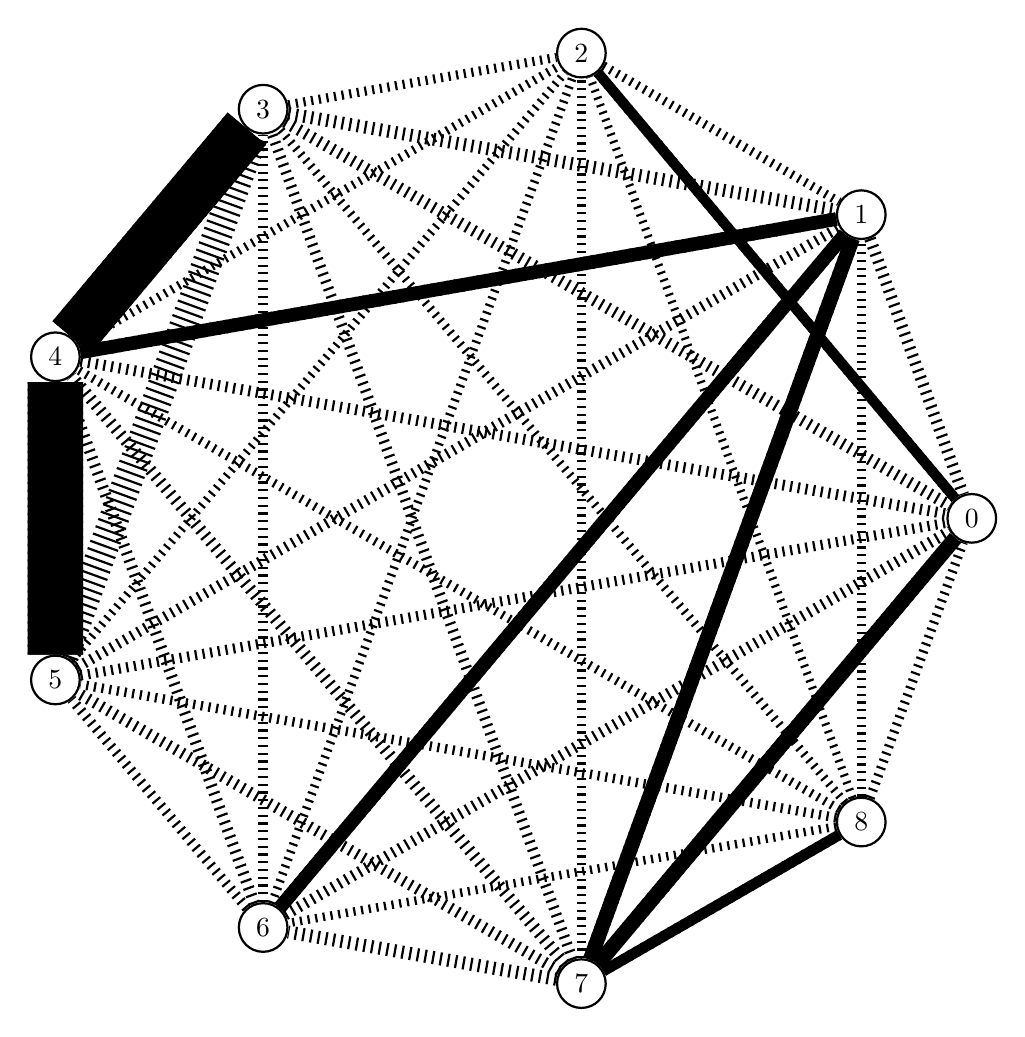
\begin{tikzpicture}[scale=1.5,auto,swap]

  % define the round nodes
  \foreach \pos/\name/\label in {
    {(4.0,0.0)/0/0a}, 
    {(3.06417777247591,2.57115043874616)/1/1a},
    {(0.694592710667722,3.93923101204883)/2/2a},
    {(-2.0,3.46410161513775)/3/3a},
    {(-3.75877048314363,1.36808057330267)/4/4a},
    {(-3.75877048314363,-1.36808057330267)/5/5a},
    {(-2.0,-3.46410161513775)/6/6a},
    {(0.69459271066772,-3.93923101204883)/7/7a},
    {(3.06417777247591,-2.57115043874616)/8/8a}}
    \node[vertex] (\label) at \pos {$\name$} ;

  %spanning tree, full edges, width proportional to the dependency
	
  \path[hi, line width=5.40]  (7a)  -- (0a);
  \path[hi, line width=5.30]  (7a)  -- (1a);
  \path[hi, line width=4.99]  (6a)  -- (1a);
  \path[hi, line width=4.92]  (4a)  -- (1a);
  \path[hi, line width=20.00]  (5a)  -- (4a);
  \path[hi, line width=18.12]  (4a)  -- (3a);
  \path[hi, line width=3.88]  (8a)  -- (7a);
  \path[hi, line width=3.71]  (2a)  -- (0a);

  % rest of edges, dotted

  \path[lo, line width=4.24]  (1a)  -- (0a);
  \path[lo, line width=3.71]  (2a)  -- (0a);
  \path[lo, line width=3.25]  (2a)  -- (1a);
  \path[lo, line width=4.33]  (3a)  -- (0a);
  \path[lo, line width=4.68]  (3a)  -- (1a);
  \path[lo, line width=3.31]  (3a)  -- (2a);
  \path[lo, line width=3.94]  (4a)  -- (0a);
  \path[lo, line width=4.92]  (4a)  -- (1a);
  \path[lo, line width=3.19]  (4a)  -- (2a);
  \path[lo, line width=18.12]  (4a)  -- (3a);
  \path[lo, line width=3.65]  (5a)  -- (0a);
  \path[lo, line width=3.84]  (5a)  -- (1a);
  \path[lo, line width=3.03]  (5a)  -- (2a);
  \path[lo, line width=10.70]  (5a)  -- (3a);
  \path[lo, line width=20.00]  (5a)  -- (4a);
  \path[lo, line width=4.08]  (6a)  -- (0a);
  \path[lo, line width=4.99]  (6a)  -- (1a);
  \path[lo, line width=3.18]  (6a)  -- (2a);
  \path[lo, line width=3.87]  (6a)  -- (3a);
  \path[lo, line width=4.12]  (6a)  -- (4a);
  \path[lo, line width=3.69]  (6a)  -- (5a);
  \path[lo, line width=5.40]  (7a)  -- (0a);
  \path[lo, line width=5.30]  (7a)  -- (1a);
  \path[lo, line width=3.12]  (7a)  -- (2a);
  \path[lo, line width=3.90]  (7a)  -- (3a);
  \path[lo, line width=4.40]  (7a)  -- (4a);
  \path[lo, line width=4.15]  (7a)  -- (5a);
  \path[lo, line width=4.75]  (7a)  -- (6a);
  \path[lo, line width=3.43]  (8a)  -- (0a);
  \path[lo, line width=3.06]  (8a)  -- (1a);
  \path[lo, line width=3.00]  (8a)  -- (2a);
  \path[lo, line width=3.15]  (8a)  -- (3a);
  \path[lo, line width=3.22]  (8a)  -- (4a);
  \path[lo, line width=3.44]  (8a)  -- (5a);
  \path[lo, line width=3.09]  (8a)  -- (6a);
  \path[lo, line width=3.88]  (8a)  -- (7a);

  
  %bended lines to the left or right
  %\path[hi] (1a) to[bend left=30] (5a);
  %\path[lo] (2a) to[bend right=30] (4a);
\end{tikzpicture}
\caption{The network of dependencies for our 9 variables. The width of each
edge is proportional to the dependency between the 2 nodes. The spanning tree
is drawn using full lines, while the other edges are drawn using dotted lines.}
\end{figure}

\end{document}